\renewcommand{\BrainFuckChapter}{%
  {-}{[}{-}{-}{-}{-}{-}{-}{-}{>}{+}{<}{]}{>}{.}{+}{[}{-}{-}{-}{>}{+}{<}{]}{>}{.}{+}{+}{+}{+}{+}{+}{.}{-}{-}{.}{-}{-}{-}{.}{-}{-}{-}{-}{-}{-}{-}{-}{-}{-}{-}{.}{-}{-}{[}{-}{-}{-}{>}{+}{<}{]}{>}{-}{.}{+}{[}{-}{>}{+}
  {+}{+}{<}{]}{>}{+}{.}{-}{[}{-}{-}{-}{>}{+}{<}{]}{>}{-}{-}{.}{-}{-}{-}{-}{-}{-}{-}{-}{-}{-}{-}{.}{+}{+}{+}{+}{+}{+}{.}{-}{.}{-}{>}{<}{>}{>}{+}{+}{>}{>}{+}{<}{-}{-}{>}{-}{<}{<}{+}{<}{>}{>}{+}{>}{-}{<}{<}{-}{+}{+}
  {-}{>}{-}{-}{+}{+}{<}{>}{+}{-}{<}{>}{+}{>}{<}{>}{-}{<}{>}{<}{-}{+}{-}{<}{+}{>}{>}{<}{>}{-}{-}{-}{-}{>}{>}{<}{-}{>}{+}{-}{-}{<}{<}{>}{-}{>}{-}{>}{>}{<}{<}{-}{-}{+}{<}{<}{+}{-}{<}{>}{<}{+}{+}{-}{<}{+}{<}{<}{-}{<}
}
\renewcommand{\LifeChapter}{y}
%%%%%%%%%%% Sprinkler Example Stuff%%%%%%%%%%%%%
\colorlet{grass}{clrd!80!green}

\tikzstyle{joint}=[cross out,rotate=45,line width=1 pt,draw=Black]
\tikzstyle{sensor}=[cross out,draw=Black,line width=1 pt,align=center,inner sep=0pt,minimum size=0.15cm,font=\tiny]
\tikzstyle{sprinkler}=[circle,draw=Black,line width=1.8 pt,align=center,inner sep=0pt,minimum size=0.2cm,font=\tiny]
\tikzstyle{radius}=[circle, dashed,draw=MidnightBlue,minimum size=1.5cm,line width=0.2 pt,align=center,font=\tiny]


\newenvironment{irrigationexample-perspective}{
  \begin{scope}[
    yshift=45,every node/.append style={
      yslant=0.5,xslant=-1},yslant=0.5,xslant=-1]
  }{
  \end{scope}
}

\newenvironment{irrigationexample-base}{
  \begin{irrigationexample-perspective}
    \fill[fill=grass,rounded corners=2em] (-1,-1) rectangle (3,3);
    \draw[opacity=0.1,step=1.0,black,thin] (-1,-1) grid (3,3);

  }{
  \end{irrigationexample-perspective}
}

\newenvironment{irrigationexample-sprinklers}{
  \begin{irrigationexample-base}
    \node [style=sprinkler] (s1) at (0, 2) {};
    \node [style=sprinkler] (s2) at (1, 2) {};
    \node [style=sprinkler] (s3) at (2, 2) {};
    \node [style=sprinkler] (s4) at (0, 1) {};
    \node [style=sprinkler] (s5) at (1, 1) {};
    \node [style=sprinkler] (s6) at (2, 1) {};
    \node [style=sprinkler] (s7) at (0, 0) {};
    \node [style=sprinkler] (s8) at (1, 0) {};
    \node [style=sprinkler] (s9) at (2, 0) {};
  }{
  \end{irrigationexample-base}
}

\newenvironment{irrigationexample-pipes}{
  \begin{irrigationexample-sprinklers}
    \node [style=joint] (sup) at (0, -1) {};

    \draw[thick] (s4) -- (s1) node[inner sep=0em, pos=0.5] (p1) {};
    \draw[thick] (s7) -- (s4) node[inner sep=0em, pos=0.5] (p2) {};
    \draw[thick] (sup) -- (s7)node[inner sep=0em, pos=0.5] (p3) {};
    \draw[thick] (s7) -- (s8) node[inner sep=0em, pos=0.5] (p4) {};
    \draw[thick] (s5) -- (s2) node[inner sep=0em, pos=0.5] (p5) {};
    \draw[thick] (s8) -- (s5) node[inner sep=0em, pos=0.5] (p6) {};
    \draw[thick] (s2) -- (s3) node[inner sep=0em, pos=0.5] (p7) {};
    \draw[thick] (s8) -- (s9) node[inner sep=0em, pos=0.5] (p8) {};
    \draw[thick] (s9) -- (s6) node[inner sep=0em, pos=0.5] (p9) {};
  }{
  \end{irrigationexample-sprinklers}
}


\newenvironment{irrigationexample-fuzzyerrors-continuous}{
  \begin{irrigationexample-perspective}
    \begin{scope}[transparency group]
      \clip[rounded corners=2em] (-1,-1) rectangle (3,3);
      \fill[grass,fill,rounded corners=2em] (-1,-1) rectangle (3,3);

      %\shade[shading=radial, inner color=brown, outer color=green, rounded  corners=2em] (-1,-4) rectangle (3,3);
      \fill[brown, path fading=fade out] (-1, -1) circle (6);
    \end{scope}
    \draw[opacity=0.1,step=1.0,black,thin] (-1,-1) grid (3,3);
  }{
  \end{irrigationexample-perspective}
}

\newenvironment{irrigationexample-fuzzyerrors-discrete}{
  \begin{irrigationexample-perspective}
    \begin{scope}
      \clip[rounded corners=2em] (-1,-1) rectangle (3,3);
      \fill[grass,fill,rounded corners=2em] (-1,-1) rectangle (3,3);

      \fill[brown] (-1,-1) rectangle (1,1);


    \end{scope}
    \draw[opacity=0.1,step=1.0,black,thin] (-1,-1) grid (3,3);

}{
  \end{irrigationexample-perspective}
}


\chapter{Introduction}
\label{sec:introduction}

Modern society is increasingly dependent on technology and, with the
appearance of low-cost computing environments, this dependency has
experienced an exponential growth.
%
Within a half-century span, computers evolved from a state where they
were only able to interact with nearby systems to the point where they
can communicate within a matter of seconds despite their distance
\citep{Allan01,Polsson}.
%
Furthermore, with the availability of low-cost high-speed
interconnections, software systems grew to global scales and gradually
infiltrated most aspects of the modern life style.

The rapid growth of software systems in terms of both size and number
happens mainly due to the fact that computers are an extremely
versatile tool, which can be used to more efficiently solve a large
variety of tasks in different domains.
%
One side effect of the large scope of software systems is the increase
in complexity \citep{Horn01}.
%
The rise in complexity almost unavoidably leads to a growing number of
bugs which, in turn, can eventually cause errors/failures
\citep{Salehie05}.


When unexpected behavior is observed, developers need to identify the
root cause(s) that made the system deviate from its intended behavior.
%
This task (also known as software debugging, fault localization, or
error diagnosis) is the most time-intensive and expensive phase of the
software development cycle \citep{Hailpern02}, and has been a concern
since the beginning of computer history\footnote{In 1946, the term bug
  was first used in the scope of computer science by Grace Hopper to
  document a problem in the Mark II computer.  In fact, the source of
  the problem was an actual bug (more specifically a moth) that was
  trapped in a relay, impeding its correct functioning.}.
%
In fact, it was estimated that the global cost of debugging software
has risen to \$312 billion annually\footnote{ University of
  Cambridge, "Financial content: Cambridge University study states
  software bugs cost economy \$312 billion per year",
  \url{http://www.prweb.com/releases/2013/1/prweb10298185.htm},
  accessed October 06, 2015.}.
%
To put this value into perspective, that is equivalent to the cost of
$729$ ``Airbus A380'' aircrafts\footnote{\$428 million per unit,
  \url{https://en.wikipedia.org/wiki/Airbus_A380}, accessed October
  06, 2015.}.

The high cost of debugging software is related to the fact that the
process of detecting, locating and fixing faults is both non-trivial
and error-prone.
%
It was estimated that a great share of the development resources,
easily ranging from $50\%$ to $70\%$, is normally assigned to software
testing and diagnosis \citep{Hailpern02} and that even experienced
developers are wrong almost $90\%$ of the time in their initial
guesses about the the faults' locations \citep{Ko08}.


To ease this process several diagnostic tools have been proposed (see
\Cref{ch:related-work} for examples).
%
Despite the improvement that such development-time diagnostic-related
tools represent, it remains practically impossible to create faultless
systems.
%
Acknowledging this fact, the concept of self-healing system has been
proposed.
%
Self-healing systems have the goal of improving their
dependability\footnote{According to \citep{Avizienis04}, dependability
  is an integrating concept that encompasses availability (readiness
  for correct service), reliability (continuity of correct service),
  safety (absence of catastrophic consequences on the users and the
  environment), integrity (absence of improper systems alterations)
  and maintainability (ability to undergo modifications and repairs).}
at run-time while reducing human intervention by employing mechanisms
that either prevent or solve eventual errors \citep{Ghosh07}.
%
In \citep{Psaier11}, the authors summarize the concept of self-healing
system as follows (\Cref{fig:introduction:self-healing}):
%
\vspace{-1em}
\begin{quote}
  ``The reason for enhancing a system with self-healing properties is
  to achieve continuous availability.
  %
  Compensating the dynamics of a running system, self-healing
  techniques momentarily are in charge of the maintenance of health.
  Enduring continuity includes resilience against intended, necessary
  adaptations and unintentional, arbitrary behavior.
  %
  Self-healing implementations work by detecting disruptions,
  diagnosing failure root cause and deriving a remedy, and recovering
  with a sound strategy.
  %
  Additionally, to the accuracy of the essential sensor and actuator
  infrastructure, the success depends on timely detection of system
  misbehavior.
  %
  This is only possible by continuously analyzing the sensed data as
  well as observing the results of necessary adaptation actions.
  %
  The system design leads to a control loop similar assembly.
  %
  An environment dependent and preferably adaptable set of policies
  support remedy decisions.
  %
  Possible policies include simple sets of event dependent
  instructions but also extended AI estimations supporting the
  resolution of previously unknown faults.''
\end{quote}%
\penalty10000
\vspace{-0.1em}
\begin{figure}[!ht]
  \scalebox{0.85}{
    \begin{tikzpicture}
      \tikzstyle{common}=[draw,font=\footnotesize,align=center,anchor=west,rounded
      corners=0.1cm, inner sep=0.2cm];

      \tikzstyle{sources}=[minimum width=3.5cm, common];
      \tikzstyle{props}=[minimum width=2.2cm,common];

      \tikzstyle{every node}=[sources];

      \node[fill=clrb](ac) at (0,0){Autonomic\\Computing \\ \citep{IBM06}};
      \node[fill=clrb,below = 1cm of ac](sas){Self-Adaptive\\Systems\\ \citep{Laddaga03}};
      \node[anchor=west,fill=clrb,below = 1cm of sas](fts){Fault-Tolerant\\Systems\\ \citep{Pierce65}};

      \node[fill=clrb,above right = -0.1cm and 0.5cm of fts](sss){
        Self-Stabilizing\\Systems  \\\citep{Dijkstra82}};
      \node[fill=clrb,below = 1.3cm of sss](ss){
        Survivable\\Systems \\ \citep{Linger98}};


      \tikzstyle{every node}=[common];
      \node[fill=clrb,ultra thick,fill=clra,font=\bfseries,below right= -0.6cm and 2.6cm of ac](shs){Self-Healing\\Systems};

      \draw (ac) edge[->,out=0,in=-180] (shs.west);
      \draw (sas) edge[->,out=0,in=-180]  (shs.west);
      \draw (fts) edge[->,out=0,in=-180]  (sss.west);
      \draw (fts) edge[->,out=0,in=-180]  (ss.west);
      \draw (sss) edge[->,out=30,in=-90]  (shs.south);
      \draw (ss) edge[->,out=30,in=-90] (shs.south);


      \tikzstyle{every node}=[props];


      \node[fill=clrc,above right = 0cm and 1cm of shs](vis){Vision};
      \node[fill=clrc,below = 1.25cm of vis](obj){Objectives};


      \node[fill=clrc,right = 0.7cm of vis](ca){Continuous\\Availability};
      \node[fill=clrc,below = 0.2cm of ca](mh){Maintenance\\of Health};
      \node[fill=clrc,below = 0.2cm of mh](sur){Survivability};



      \node[fill=clrc,below = 0.2cm of sur](det){Detecting};
      \node[fill=clrc,below = 0.2cm of det](dia){Diagnosing};
      \node[fill=clrc,below = 0.2cm of dia](rec){Recovery};
      \node[fill=clrc,left = of dia](att){Attributes};

      \node[fill=clrc,below = 0.2cm of rec](cl){Closed-loop};
      \node[fill=clrc,below = 0.2cm of cl](pol){Policies};
      \node[fill=clrc,below = 1.7cm of att](mea){Means};

      \draw (shs) edge[->,out=0,in=-180] (vis.west);
      \draw (shs) edge[->,out=0,in=-180] (obj.west);
      \draw (shs) edge[->,out=-60,in=180] (att.west);
      \draw (shs) edge[->,out=-60,in=140] (mea.west);


      \draw (vis) edge[->,out=0,in=-180] (ca.west);
      \draw (obj) edge[->,out=0,in=-180] (mh.west);
      \draw (obj) edge[->,out=0,in=-180] (sur.west);
      \draw (att) edge[->,out=0,in=-180] (det.west);
      \draw (att) edge[->,out=0,in=-180] (dia.west);
      \draw (att) edge[->,out=0,in=-180] (rec.west);
      \draw (mea) edge[->,out=0,in=-180] (cl.west);
      \draw (mea) edge[->,out=0,in=-180] (pol.west);

    \end{tikzpicture}
  }
  \caption{Relations and properties of self-healing research (adapted
    from \citep{Psaier11})}
  \label{fig:introduction:self-healing}
\end{figure}
\penalty-10000


The self-healing concept is in fact a specialization of a broader
concept, called autonomic computing \citep{Kephart03}.
%
To implement an autonomic system, \emph{IBM} suggests a reference
model for autonomic control loops \citep{IBM06}, referred to as the
\ac{MAPE-K} control loop and is depicted in
\Cref{fig:intro:MAPE-K-control-loop}.
%
In the \ac{MAPE-K} autonomic loop, the managed resource represents
any software or hardware resource that is given autonomic behavior by
coupling it with an autonomic manager.
%
In a practice, the managed resource can be, for instance, a web
server, a database, an operating system, a cluster of machines, a hard
drive, a wired or wireless network, \etc.

\begin{figure}[!ht]
  \includegraphics[width=0.6\columnwidth,page=13]{figures/introduction/figures/main.pdf}
  \caption{\acs{MAPE-K} control loop\label{fig:intro:MAPE-K-control-loop} }
\end{figure}




In the context of self-healing systems, the \emph{monitor} component
determines whether the system is in degraded or erroneous state,
through the information collected by the managed resource's sensors
(also known as probes or gauges \citep{Garlan01}).
%
The \emph{analyzer} component is responsible for pinpointing the
probable source(s) of system errors.
%
The \emph{plan} component creates a repair plan targeted at returning
the system to an operational state.
%
The \emph{executor} component implements the repair plan, by using a set of
system effectors that carry out changes to the managed resource.
%
The change implemented by the \emph{effectors} can be coarse-grained
(\eg, adding or removing servers to a web server cluster
\citep{Garlan04}) or fine-grained (\eg, changing configuration
parameters in a web server) \citep{Bigus02}.
%
The \emph{knowledge} component collects the knowledge produced by all
the aforementioned components and stores it for future use.



In this thesis, our focus is on the analyzer component of the
\ac{MAPE-K} control loop.
%
Our goal is to create an automatic diagnostic framework for run-time
systems.
%
Even though several diagnostic approaches have been proposed the large
majority is either too specific to a particular application (\eg,
\citep{Chao04,Mohammadi07,Kasick10,Tan10,Shvachko10}) or too costly
(\eg, \citep{Reiter87,Kleer87,Mayer03,Wotawa02}).
%
In contrast to the existent approaches, we aim at creating a
diagnostic framework meeting the following criteria:
%
\begin{itemize}[nolistsep]
\item It must be ``general purpose'':
  \begin{itemize}
  \item It must be usable in a large variety of systems.
  \item It must be possible to add new components to the managed
    resource without altering the diagnostic framework.
  \item It must handle different instrumentation granularities.
  \end{itemize}

\item It must be ``scalable'':
  \begin{itemize}
  \item It must be able to handle systems with large number of
    components.
  \end{itemize}

\item It must be ``accurate''
\end{itemize}
%

To achieve our goal while meeting the aforementioned criteria, we
improve over a development-time diagnostic technique called \ac{SFL}.
%
\ac{SFL} uses a high-level abstraction of the system under analysis,
making it, in principle, usable in a large diversity of scenarios.
%
The only requirements to use \ac{SFL} in a real-world scenario are
that
\begin{inparaenum}[(1)]
\item the system's activity must be divisible into transactions,
\item the correctness of each transaction must be evaluable,
\item the components' activations must be observable and
\item it must be possible to associate the components' activity with
  the corresponding transactions.
\end{inparaenum}

The high-level abstraction implies that a large amount of the
diagnostic complexity is traded-off for accuracy.
%
Even though \ac{SFL} is less accurate than some existing diagnostic
approaches (\eg, \citep{Reiter87,Kleer87,Mayer03,Wotawa02}), it is able to
scale to large systems where heavier approaches are not usable.
%
Furthermore, given enough diversity in the observations, \ac{SFL}
tends to be accurate enough for practical
purposes \citep{Santelices09,Abreu09f}.


In the remainder of this chapter we further discuss the scope of our
work.
%
In \CrefPageParen{sec:intro:diagnostic-problem}, we describe the
diagnostic problem.
%
In \CrefPageParen{sec:intro:SFL}, we present the state-of-the-art
\ac{SFL} approach for development-time diagnosis.
%
In \CrefPageParen{sec:intro:research-goals}, we discuss our research
goals.
%
In \CrefPageParen{sec:intro:origin-of-chapters}, we present the origin of
chapters.
%
Finally, in \CrefPageParen{sec:intro:outline}, we present the thesis
outline.

\section{Diagnostic Problem}
\label{sec:intro:diagnostic-problem}
In general terms, a diagnostic problem occurs whenever the behavior of
a particular system (natural or artificial) deviates from the expected
behavior \citep{Reiter87,Kleer92}.
%
The challenge consists in finding the true root causes of such
abnormal behavior.
%

In our work we use the taxonomy proposed by \citep{Avizienis04}:
\begin{itemize}
\item An \textbf{error} is an incorrect system state that may cause a
  failure.
\item A \textbf{failure}, is the observable manifestation of an error:
  an error becomes a failure when it propagates to the system's output.
\item A \textbf{fault/bug} is the cause of an error in the system.
\end{itemize}

\begin{figure}[h!]
  \lstinputlisting[
  language=python,
  xleftmargin=.1\textwidth,
  xrightmargin=.1\textwidth,
  ]{figures/introduction/error.py}
  \caption{Bug example\label{fig:bugexample}}
\end{figure}

To illustrate these concepts, take for instance the three Python
functions presented in \Cref{fig:bugexample}.
%
The purpose of function $\fn{f\_to\_c}$ is to convert a temperature
from \textit{Fahrenheit} degrees to \textit{Celsius}.
%
Since the whole operation is performed using integer arithmetic, the
implementation is faulty and may compute erroneous results.
%
Function $\fn{is\_freezing\_f}$, which is implemented by daisy
chaining functions $\fn{f\_to\_c}$ and $\fn{is\_freezing\_c}$, should
return $\mTrue$ if the input value (in \textit{Fahrenheit}) is
below water's freezing point and $\mFalse$ otherwise.

\begin{figure}[!ht]
  \begin{tabular}{c|r@{}@{}lr@{}l|cc|c}
    % \cline{2-7}
    \multicolumn{1}{c|}{} & \multicolumn{4}{c|}{$\fn{f\_to\_c}$} & \multicolumn{2}{c|}{$\fn{is\_freezing\_f}$}                                                           \\
    \hline
    Input                 & \multicolumn{2}{c}{Expected}         & \multicolumn{2}{c|}{Observed} & Expected & Observed    & Outcome                                      \\
    \hline
    $31^{\circ} F$        & $-0.55_{5}$                          & $^{\circ}C$                   & $-1$     & $^{\circ}C$ & $\mTrue$  & $\mTrue$ & Error   \\
    $32^{\circ} F$        & $0$                                  & $^{\circ}C$                   & $0$      & $^{\circ}C$ & $\mTrue$  & $\mTrue$ & Nominal \\
    $33^{\circ} F$        & $0.55_{5}$                           & $^{\circ}C$                   & $0$      & $^{\circ}C$ & $\mFalse$ & $\mTrue$ & Failure \\
  \end{tabular}

  \caption{$\fn{is\_freezing\_f}$ function trace\label{tab:trace}}
\end{figure}
By analyzing \Cref{tab:trace}, we can see that for $32^\circ F$ the
function \textit{$\fn{is\_freezing\_f}$} not only works as expected
but also does not activate the fault (\ie, the result of
$\fn{f\_to\_c}$ is correct).
%
For $31^\circ F$, despite activating the fault (\ie, the result of
$\fn{f\_to\_c}$ is not correct), the aggregate result of both
functions is correct due to the fact that function
$\fn{is\_freezing\_c}$ masks the error.
%
Finally, for $33^\circ F$ the fault is activated and the error
propagates to the system output, delivering an incorrect result.

A prerequisite to diagnose a system is that the occurrence of
errors/failures is detected.
%
The process of observing the system state and deciding whether or not
it satisfies the system's specification is known as the oracle
problem.


The approaches to solve the diagnostic problem can be broadly divided
in two groups: heuristic and model based diagnosis (also known as
diagnosis from first principles).

\subsection{Heuristic-based Diagnosis}
\label{sec:intro:heuristic-diagnosis}
Heuristic-based diagnosis approaches are focused on encoding expert
knowledge generated by previous diagnostic experience to more
efficiently address future diagnostic problems.
%
In such diagnostic systems, the diagnostic reasoning is greatly based
upon the observed error symptoms and the possible (known) solutions to
such symptoms.
%
A consequence of this type of reasoning is that the structure of the
system under analysis is only weakly represented, if present at all.
%
While such diagnostic systems are effective in diagnosing known
abnormalities, they tend to fail whenever new error symptoms emerge.

\begin{figure}[ht]
  \begin{subfigure}{\columnwidth}
    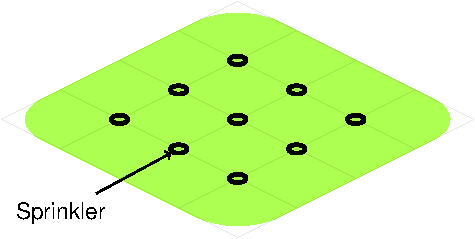
\includegraphics[page=1]{figures/introduction/figures/main.pdf}
    \caption{Sprinklers\label{fig:intro:irrigation-example-sprinklers}}
  \end{subfigure}


  \begin{subfigure}{\columnwidth}
    \includegraphics[page=2]{figures/introduction/figures/main.pdf}
    \caption{Piping\label{fig:intro:irrigation-example-piping}}
  \end{subfigure}
  \caption{Irrigation system example\label{fig:intro:irrigation-example}}
\end{figure}

As an illustrative example, consider an irrigation system with the
additional goal of guaranteeing that irrigation problems are
automatically detected and diagnosed.
%
For the example shown in
\Cref{fig:intro:irrigation-example-sprinklers}, one could use
peer-similarity to accomplish the self-diagnosis goal.
%
The usage of peer-similarity requires that all
components in the system behave similarly with regard to a set of
metrics and the presence of outlier metric values implies the
occurrence of errors in the corresponding components
\citep{Kasick10,Shvachko10,Tan10}.
%
Assuming that, for instance, the water pressure or consumption for
each sprinkler is observable, substantial variations in such metrics
among the system's sprinklers would signal a sprinkler failure.


Even though this approach would most likely perform well in the
described system, in a system where the sprinklers operate at
different pressures or have different water consumption rates the
outlier detection would be too inaccurate.
%
Furthermore, if all the sprinklers in the system fail similarly, this
particular approach may fail to detect and, consequently, to diagnose
the errors.

Another problem with the aforementioned approach is related to the
fact that, to meet the similarity requirement, the abstraction of the
system neglects the existence of important components and may result
in poor diagnostic quality.
%
Considering the fact that the sprinklers are fed by a piping system,
as depicted in \Cref{fig:intro:irrigation-example-piping}, the
observation of an error symptom in a sprinkler does not necessarily
mean that the problem occurred there.
%
In practice, the symptom of low water pressure may be due to water
shortage, piping failure, and/or sprinkler failure.

Finally, consider a situation in which the state of the sprinklers is
not directly observable but instead the system is equipped with
humidity sensors, placed at arbitrary positions in the field, as shown
in \Cref{fig:intro:example2}.
%
As the state of the system's components is not available, the
peer-similarity technique is no longer usable.


\begin{figure}[ht]
  \includegraphics[page=3]{figures/introduction/figures/main.pdf}
  \caption{Irrigation system example -- Sensors\label{fig:intro:example2}}
\end{figure}

Another example of this type of diagnostic approach is the so-called
medical diagnostic guidelines.
%
Even though such guidelines effectively enhance both diagnostic
accuracy and efficiency for common diseases, they fail in the presence
of unknown symptoms/diseases (\eg, a patient with a green glowing
eye).

Even though apparently unrelated to the computer science domain, the
previous examples show the potential problems related to heuristic
diagnostic techniques.
%
Establishing a parallel with software, we see that software systems
are mostly composed of heterogeneous sets of components with, almost
inevitably, different degrees of state observability thus strongly
limiting the scope of application of existing diagnostic heuristics
over different systems \citep{Salehie05}.

\subsection{\acl{MBD}}
\label{sec:intro:model-based-diagnosis}
\ac{MBD} approaches focus on encoding the structure and expected
behavior of the system under analysis which, together with
observations of the system's behavior, are used to perform the
diagnostic reasoning \citep{Kleer87,Reiter87}.
%
\begin{definition}[Model-based Diagnostic System]
  A model-based diagnostic system $\DS$ is defined as the triple
  $\DS = (\SD, \COMPS,\OBS)$ , where:
  \begin{itemize}
  \item $\SD$ is a propositional theory describing the behavior of the system
  \item $\COMPS = \set{c_1 , \ldots, c_M }$ is a set of components in $\SD$
  \item $\OBS$ is a set of observable variables in $\SD$
  \end{itemize}
\end{definition}


The existence of such a model enables the diagnostic system to
successfully cope (from a theoretical point-of-view) with new error
symptoms (such as the patient with the glowing eye).
%
Whenever the observed system behavior for a particular scenario (\ie,
a specific assignment over variables in $OBS$) conflicts with the
behavior predicted by the model $SD$, the diagnostic reasoning
revolves around finding sets of components that, by assuming their
faultiness, would explain the erroneous behavior.

To guarantee generality, \ac{MBD} algorithms reason in terms of
conflicts.
%
Informally, a conflict represents a set of components that cannot be
simultaneously healthy to explain the observed erroneous behavior.

\begin{definition}[h-literal]
  An h-literal, denotes the component's health.
  %
  The positive h-literal $h$ corresponds to a healthy component
  whereas, the negative h-literal $\neg h$ corresponds to an
  unhealthy one.
\end{definition}

\begin{definition}[Conflict]
  Let $\fn{HL}^+(C) = \bigwedge_{j \in C} h_j$ be the conjunction of
  positive h-literals for a set of components $C \subseteq \COMPS$ and
  $obs$ an observation term over variables in $\OBS$.  $C$ is a
  conflict for $(\DS, obs)$ if and only if:
  \begin{equation}
    \SD \wedge obs \wedge \fn{HL}^+(C)
  \end{equation}
  is inconsistent.
\end{definition}

In other words, a conflict is a set of components that cannot be
simultaneously healthy for the observed erroneous behavior
to occur.

\begin{definition}[Diagnostic Candidate]
  \label{def:intro:candidate}
  Let $C \subseteq \COMPS$ be a set of components.  We define $d(C)$
  to be the conjunction:
  \begin{equation}
    \Big(\bigwedge_{m \in C} \neg h_m\Big) \wedge
    \Big(\bigwedge_{m \in \COMPS \setminus C}  h_m\Big)
  \end{equation}
  Given an observation term $obs$ over variables in $\OBS$, a
  diagnostic candidate for $\DS$ is a conjunction $d(C)$
  such that:
  \begin{equation}
    \SD \wedge obs \wedge d(C)
  \end{equation}
  is consistent.

  In the remainder we refer to $d(C)$ simply as $d$, which
  we identify with the set $C$.
\end{definition}

In this context, a diagnostic candidate is thereby a set of components
that is conjectured to be unhealthy, resolving all conflicts entailed
by $\SD \wedge obs$.


A problem with the above definition is related to the fact that a
candidate $d$ containing all of the system's components (\ie, $d =
\COMPS$) always resolves every conflict by $\SD \wedge obs$.
%
Intuitively, this is equivalent to saying that the whole system is
faulty which, in practice, is not a very helpful conclusion.
%
To apply the concept of a diagnostic candidate to real systems with
success, one must refine the definition so that the candidate contains
the minimum number of components while still solving all the
conflicts.

\begin{definition}[Minimal Diagnostic Candidate]
  \label{def:intro:minimal-candidate}
  A candidate $d$ is minimal if and only if
  $\nexists_{d^\prime} : d^\prime \subset d$ such that $d^\prime$ is a diagnostic
  candidate.
\end{definition}

The end result of the diagnostic reasoning is the diagnostic
report.
%
A diagnostic report features a set of explanations for the erroneous
behavior (\ie, the diagnostic candidates) as well as a measure of how
likely each explanation is.
%
The process of calculating a diagnostic report can be broadly divided
in two stages, as depicted in \Cref{fig:intro:diagnostic-process}.

\begin{figure}[ht]
  \includegraphics[page=4]{figures/introduction/figures/main.pdf}
  \caption{Diagnostic process\label{fig:intro:diagnostic-process}}
\end{figure}

\begin{definition}[Diagnostic Report]
  \label{def:intro:diagnostic-report}

  A diagnostic report
  $\diag = \left(d_1, \dots, d_k, \dots, d_K\right)$ is an ordered set
  of $K$ diagnostic candidates, such that:
  \begin{equation}
    \forall_{d_k\in \diag} : \pr{d_k \mid obs} \geq \pr{d_{k+1} \mid obs}
  \end{equation}
\end{definition}


\section{\acl{SFL}}
\label{sec:intro:SFL}
A limitation of traditional \ac{MBD} approaches is the necessity of a
detailed system model which, in practice and due to the large
complexity of modern computer systems, normally entails a large
modeling effort/cost, thus narrowing its range of application
\citep{Pietersma06,Horn01}.
%
To overcome the complexity of creating precise system models,
\acf{SFL}\footnote{For simplicity and unless stated otherwise, we use
  the acronym \ac{SFL} to refer to a particular \ac{SFL} approach
  known as Spectrum-based Reasoning for Fault Localization.
  %
  In \CrefPageParen{sec:related-work:similarity-based-SFL} an
  alternative and more common \ac{SFL} approach is presented.}
approaches were proposed \citep{Abreu09a,Kleer09,Casanova13}.
%
Instead of relying on a fine grained model of the system (\ie,
$SD \in DS$) to generate conflict sets, \ac{SFL} infer conflicts by
performing a dynamic analysis of the system.

To apply \ac{SFL} to a system, it must be abstracted in terms of two
general concepts: component, and transaction.
%
A component is an element of the system that, for diagnostic purposes,
is considered to be atomic\footnote{In a software environment, a
  component can be for instance a statement, a function, a class, a
  service, \etc.}.
%
A transaction is a set of component activations that
\begin{inparaenum}[(1)]
\item share a common goal, and
\item the correctness of the provided service can be verified.
\end{inparaenum}
%
The error detection mechanism, from a \ac{SFL} perspective, is treated
as a black box.

To gather all the required information to perform diagnosis, the
system under analysis must be instrumented (see
\Cref{sec:related-work:code-coverage}).
%
The instrumentation's output, commonly known as
spectrum \citep{Harrold98}, is defined as the
pair $(A, e)$ (\Cref{fig:intro:sfl-matrix}), where:

\begin{itemize}
\item $A$ (\textbf{activity matrix}) encodes the involvement of
  components in transactions.
\item $e$ (\textbf{error vector}) encodes the correctness of each
  individual transaction.
\end{itemize}

\begin{figure}[!ht]
  \begin{equation*}
    \stackrel{\mbox{activity matrix}}{%
      \begin{bmatrix}
        A_{11} & A_{12} & \cdots & A_{1M} \\
        A_{21} & A_{22} & \cdots & A_{2M} \\
        \vdots & \vdots & \ddots & \vdots \\
        A_{N1} & A_{N2} & \cdots & A_{NM}
      \end{bmatrix}
    }\ \ \ \stackrel{\stackrel{\mbox{error}}{\mbox{vector}}}{%
      \begin{bmatrix}
        e_1    \\
        e_2    \\
        \vdots \\
        e_N
      \end{bmatrix}%
    }
  \end{equation*}
  \caption{Spectrum with $M$ components and $N$ transactions\label{fig:intro:sfl-matrix}}
\end{figure}

Even though several types of spectra exist, the most commonly used is
called a hit spectrum \citep{Harrold98,Yilmaz08,Santelices09}.
%
\begin{definition}[Hit Spectrum]
  \label{def:intro:hit-spectrum}
  The hit spectrum abstraction encodes the components' activity in terms
  of hit/not hit and the transactions' correctness in terms of
  pass/fail.
  %
  Using the hit spectrum abstraction, $A$ and $e$ are defined as:
  \begin{equation}
    A_{ij} = \begin{cases}
      1, & \textrm{if component $j$ was involved in transaction $i$}\\
      0, & \textrm{otherwise}
    \end{cases}
  \end{equation}
  \begin{equation}
    e_{i} = \begin{cases}
      1, & \textrm{if transaction $i$ failed}\\
      0, & \textrm{otherwise}
    \end{cases}
  \end{equation}
\end{definition}

For convenience, in this thesis we may treat $A_i$ as a set containing
the indices of all components involved in transaction $i$.
%
Formally, $A_i$ can also be defined as:
\begin{equation}
  A_{i} = \set{j \mid \textrm{if component $j$ was involved in transaction $i$}}
\end{equation}
%
Since both forms encode the same information, we can use the two forms
interchangeably.
%
Whenever we apply set operations to $A$, we are implicitly using the
set form.
%
In \Cref{fig:intro:hit-spectrum-example} an example hit
spectrum in both forms is presented.
\begin{figure}[ht]
  \begin{subfigure}{0.4\columnwidth}
    \begin{tabular}{c|ccc|c}
      \multirow{2}{*}{$i$} & \multicolumn{3}{c|}{$A$} & \multirow{2}{*}{$e$} \\
      \cline{2-4}
                           & $c_1$                    & $c_2$ & $c_3$ &      \\ \hline
      $1$                  & $1$                      & $1$   & $0$   & $1$  \\
      $2$                  & $1$                      & $0$   & $1$   & $1$  \\
      $3$                  & $1$                      & $1$   & $1$   & $0$  \\
    \end{tabular}
    \caption{Matrix form}
  \end{subfigure}
  \begin{subfigure}{0.4\columnwidth}
    \begin{tabular}{c|c|c}
      $i$                  & $A$                      & $e$                  \\\hline
      $1$                  & $\set{1,2}$              & $1$                  \\
      $2$                  & $\set{1,3}$              & $1$                  \\
      $3$                  & $\set{1,2,3}$            & $0$                  \\
    \end{tabular}
    \caption{Set form}
  \end{subfigure}
  \caption{Hit spectrum example\label{fig:intro:hit-spectrum-example}}
\end{figure}


\begin{figure}[!ht]
  \begin{subfigure}{\columnwidth}
    \includegraphics[page=5]{figures/introduction/figures/main.pdf}
    \caption{Components\label{fig:intro:example-sfl-components}}
  \end{subfigure}
  \\[2em]
  \begin{subfigure}{\columnwidth}
    \includegraphics[page=6]{figures/introduction/figures/main.pdf}
    \caption{Transaction\label{fig:intro:example-sfl-transaction}}
  \end{subfigure}
  \\[2em]
  \begin{subfigure}{\columnwidth}
    \bgroup
    \def\x{{\Large$\bullet$}}
    \setlength\tabcolsep{0.2em}
    \newcolumntype{T}{t{1.4em}}

    \begin{tabular}{T|TTTTTTTTTTTTTTTTTTT|T}
      \multirow{2}{*}{$i$} & \multicolumn{19}{c|}{$A$} & \multirow{2}{*}{$e$}                                                                                                                                                              \\\cline{2-20}
                           & $c_1$                     & $c_2$ & $c_3$ & $c_4$ & $c_5$ & $c_6$ & $c_7$ & $c_8$ & $c_9$ & $c_{10}$ & $c_{11}$ & $c_{12}$ & $c_{13}$ & $c_{14}$ & $c_{15}$ & $c_{16}$ & $c_{17}$ & $c_{18}$ & $c_{19}$ &     \\ \hline
      $1$                  & \hit                      & \hit  & \nhit & \hit  & \hit  & \nhit & \nhit & \nhit & \nhit & \hit     & \hit     & \hit     & \hit     & \hit     & \hit     & \nhit    & \nhit    & \nhit    & \hit     & \hit \\
      $2$                  & \nhit                     & \hit  & \hit  & \nhit & \hit  & \hit  & \nhit & \nhit & \nhit & \nhit    & \nhit    & \hit     & \hit     & \hit     & \hit     & \hit     & \hit     & \hit     & \hit     & \nhit \\
      $3$                  & \nhit                     & \nhit & \nhit & \hit  & \hit  & \nhit & \hit  & \hit  & \nhit & \nhit    & \hit     & \hit     & \hit     & \nhit    & \hit     & \nhit    & \nhit    & \nhit    & \hit     & \nhit \\
      $4$                  & \nhit                     & \nhit & \nhit & \nhit & \hit  & \hit  & \nhit & \hit  & \hit  & \nhit    & \nhit    & \hit     & \hit     & \nhit    & \hit     & \nhit    & \hit     & \hit     & \hit     & \hit \\
    \end{tabular}
    \egroup
    \caption{Hit spectrum (0's and 1's were replaced by ``.'' and
      ``{\Large$\bullet$}'' for
      readability)\label{fig:intro:example-sfl-spectrum}}
  \end{subfigure}
  \caption{Irrigation system example -- \acs{SFL}}
\end{figure}


To illustrate how \ac{SFL} can be used in an arbitrary system,
consider again the example in \Cref{fig:intro:example2}.
%
For this system, the set of all components is composed of $19$ elements
(\Cref{fig:intro:example-sfl-components}): $9$ sprinklers ($c_1$ through
$c_9$), $9$ piping elements ($c_{10}$ through $c_{18}$) and the water supply
($c_{19}$).
%
There are $4$ different transaction types (one for each
sensor).
%
Each of those transactions consists of the activation of all the
surrounding sprinklers as well as the piping elements used to by those
sprinklers, as depicted in \Cref{fig:intro:example-sfl-transaction}.
%
A possible approach to evaluate the success of each transaction would
be to compare the humidity value obtained by the corresponding sensor
to an arbitrary threshold interval.
%
If the humidity on the ground is either too high or too low,
the transaction fails.

Consider a scenario where, for the described system, sensors $s_1$ and
$s_4$ (see \Cref{fig:intro:example-sfl-transaction}) detect an incorrect
humidity level whereas, the remaining sensors, detect a corrected
humidity level.
%
The spectrum corresponding to this scenario is depicted in
\Cref{fig:intro:example-sfl-spectrum}.
%
The spectrum contains $4$ transactions (each transaction $i$
corresponds to the sensor $s_i$) and both transactions $1$ and $4$ are
marked as erroneous.
%
Additionally, for each transaction, all the sprinklers adjacent to the
corresponding sensor as well as the piping elements needed to feed
such sprinklers are marked as active.



In the next sub-sections we present the relevant details of existent
\ac{SFL} algorithms to solve both the candidate generation and ranking
problems.


\subsection{Candidate Generation}
\label{sec:intro:candidate-generation}
In a na\"{i}ve approach, the candidate generation problem can be
addressed by computing the power set of all components in the system
($\powSet{\COMPS}$).
%
However, as $|\set{\powSet{\COMPS}}| = 2^{\set{|\COMPS|}}$, this
approach becomes quickly ineffective.
%
In practice, rather than iterating over \emph{all} possible sets just
to find that most are not minimal or even consistent with the
observations, search algorithms are typically used to only consider
sets that meet the minimal candidate criteria (see
\Cref{def:intro:minimal-candidate}).
%

Despite the advantage of only computing minimal candidates, the
problem is still remarkably hard.
%
The calculation of minimal candidates, conceptually referred to as
hitting sets, is a problem equivalent to the \acl{MHS} problem
\citep{Reiter87}, which is known to be NP-Hard \citep{Garey90}.
%
The formal definition of the \acl{MHS} problem goes as follows:

\begin{definition}[Hitting Set]
  \label{def:intro:hitting-set}
  Given a set $U$ of $M$ elements (called the universe) and a
  collection $S$ of $N$ sets, a set $d$ is said to be a \acf{HS} of
  $(U,S)$ if and only if:
  \begin{equation}
    \label{eq:intro:hitting-set}
    \displaystyle \HS(U,S,d):= d \subseteq U \wedge \big(\forall_{s \in S}: d \cap s \not = \emptyset\big)
  \end{equation}
\end{definition}
\begin{corollary}
  If $\nexists_{s \in S} : s \cap U = \emptyset$, $U$ is a \ac{HS} of $S$.
\end{corollary}

\begin{corollary}
  \label{cor:intro:unsatisfiablity}
  If $\exists_{s \in S} : s \cap U = \emptyset$, $\HS(U,S,d)$ never holds.
\end{corollary}

\begin{corollary}
  \label{cor:intro:emptyHS}
  $d = \emptyset$ is a hitting for $S = \emptyset$.
\end{corollary}

\begin{corollary}
  \label{cor:intro:associativity}
  $\HS(U,S,d)$ is associative:
  \begin{equation}
    \displaystyle \HS(U,S,d) \wedge \HS(U^\prime,S^\prime,d^\prime) \implies
    \HS(U\cup U^\prime,S \cup S^\prime, d \cup d^\prime)
  \end{equation}
\end{corollary}

\begin{definition}[Minimal Hitting Set]
  A set $d$ is a \acf{MHS} of $(U,S)$ if and only if:
  \begin{equation}
    \label{eq:intro:minimal-hitting-set}
    \MHS(U,S,d):= \HS(U,S,d) \wedge \big(\nexists_{d^\prime \subset d}: \HS(U,S,d^\prime)\big)
  \end{equation}
  \noindent
  \ie, $d$ is a \ac{HS} and no proper subset of $d$ is a \ac{HS}.
\end{definition}
%
There may be several \acp{MHS} $d_k$ for $(U,S)$, which
constitute the \ac{MHS} collection $D$.
%
The \ac{MHS} problem consists thereby in computing $D$ for a
particular pair $(U,S)$.

Putting this definition in terms of the candidate generation problem,
the set of all components of the system ($\COMPS$) is equivalent to
the set $U$, whereas the set of all conflicts entailed by
$\SD \wedge obs$ is equivalent to $S$.
%
A \ac{MHS} for all the conflicts entailed by $\SD \wedge obs$ is, in
fact, a diagnostic candidate for $\SD \wedge obs$ \citep{Reiter87}.


Under the \ac{SFL} abstraction, a conflict occurs whenever a failed
transaction exists in the spectrum.
%
The elements of the conflict set are the components activated in such
transaction.
%
Intuitively, since the transaction failed, it follows that at least
one of the components must not be healthy for the erroneous behavior
to occur.


As an example, consider the hit spectrum in
\Cref{fig:intro:spectrum-example} for which all $2^M$ possible (but
not necessarily valid) candidates (\ie, $\powSet{\COMPS}$) are
presented in \Cref{fig:intro:hasse}.
%
For this particular spectrum, two minimal candidates/\acp{MHS} exist:
$\set{1}$ and $\set{2,3}$.
%
Even though the set $\set{1,2,3}$ is also \ac{HS}, it is not minimal
as it can be subsumed either by $\set{1}$ or $\set{2,3}$.

\begin{figure}[ht]
  \begin{subfigure}{0.4\columnwidth}
    \begin{tabular}{c|c|c}
      $i$ & $A$           & $e$ \\\hline
      $1$ & $\set{1,2}$   & $1$ \\
      $2$ & $\set{1,3}$   & $1$ \\
      $3$ & $\set{1,2,3}$ & $0$ \\
    \end{tabular}
    \caption{Hit spectrum\label{fig:intro:spectrum-example}}
  \end{subfigure}
  %
  \begin{subfigure}{0.45\columnwidth}
    \includegraphics[page=7]{figures/introduction/figures/main.pdf}
    \caption{Hasse diagram of $\powSet{\set{1,2,3}}$\label{fig:intro:hasse}}
  \end{subfigure}
  \caption{Example}
\end{figure}





Being a NP-hard problem, the usage of exhaustive search algorithms
(\eg, \citep{Reiter87,Wotawa01}), is prohibitive for most real-world
problems.
%
In order to solve the candidate generation problem in a reasonable
amount of time, approaches that relax the strict
minimality\footnote{We use the term minimal in a more liberal way due
  to mentioned relaxation. A candidate $d$ is said to be minimal if no
  other calculated candidate is contained in $d$.} constraint have
been proposed \citep{Abreu09b,Kleer92,Feldman08}.

A simplified\footnote{For simplicity, the cutoff conditions were
  omitted.} version of the state-of-the-art \ac{SFL} candidate
generation algorithm (called \staccato{}) \citep{Abreu09b} is
presented in \Cref{alg:intro:staccato} and
\Cref{fig:intro:cg-flowchart}.
%
The algorithm works in a divide and conquer fashion by, at each stage
of its execution, performing one of two different tasks (lines
\ref{alg:intro:staccato:rank},
\ref{alg:intro:staccato:S'}, and
\ref{alg:intro:staccato:rec} or
\ref{alg:intro:staccato:isminimal}--\ref{alg:intro:staccato:addD}),
depending on whether the set $d$ is a \ac{HS}.
%
As we shall shortly see, due to the algorithm's divide and conquer
nature, $d$ is a \ac{HS} whenever $S = \emptyset$.

The first task, which is triggered whenever $d$ is not a \ac{HS} (line
\ref{alg:intro:staccato:divide}), aims at dividing the initial
problem in smaller sub-problems.
%
This goal is achieved by iteratively selecting an element $j \in U$
from a heuristically\footnote{The details of chosen heuristic are
  presented in \Cref{sec:mhs2o:heuristics}. For now assume that the
  order is arbitrary and that, for every possible ordering, the
  algorithm computes the same result.} ordered set (line
\ref{alg:intro:staccato:rank}) and creating a temporary collection
$S^\prime$
containing all the sets $s \in S : j \in s$,
\ie, the sets hit by $\set{j}$ (line \ref{alg:intro:staccato:S'}).
%
Finally, the algorithm makes a recursive call to solve the sub-problem
$S \setminus S^\prime$ with set $d \cup \{j\}$ (line
\ref{alg:intro:staccato:rec}).

The second task, which occurs whenever $d$ is a \ac{HS} (line
\ref{alg:intro:staccato:conquer}), aims at collecting \acp{HS}
while guaranteeing that no \ac{HS} in $D$ has a proper subset also
contained in $D$.
%
The first step in this task is to check if $d$ is minimal (line
\ref{alg:intro:staccato:isminimal}) with regard to the already
discovered \ac{MHS} collection $D$.
%
If $d$ is minimal, all super-sets of $d$ in $D$ are purged (line
\ref{alg:intro:staccato:purge}) and, finally, $d$ is added to
$D$ (line \ref{alg:intro:staccato:addD}).

\begin{algorithm}
  \begin{description}
  \item[Inputs:]\ $(U, S, d=\emptyset, D=\emptyset)$
  \item[Output:]\ Minimal hitting set collection $D$
  \end{description}

  \begin{algorithmic}[1]
    \If{$S \not= \emptyset$}   \algorithmiccomment{\textbf{divide task}} \label{alg:intro:staccato:divide}
    \For{$j \in  \fn{Rank}(U, S)$} \label{alg:intro:staccato:rank}
    \State $S^\prime \gets \set{s \mid s \in S \wedge j \in s}$  \label{alg:intro:staccato:S'}
    \State $D \gets \fn{Staccato}(U \setminus \set{j}, S \setminus S^\prime, d \cup \set{j}, D)$  \label{alg:intro:staccato:rec}
    \EndFor
    \Else
    \algorithmiccomment{\textbf{conquer task}} \label{alg:intro:staccato:conquer}
    \If{$\nexists_{d^\prime\in D}: d^\prime\subseteq d$} \label{alg:intro:staccato:isminimal}
    \State $D \gets D \setminus \set{d^\prime \mid d^\prime \in D \wedge  d \subseteq d^\prime}$  \label{alg:intro:staccato:purge}
    \State $D \gets D \cup \set{d}$ \label{alg:intro:staccato:addD}
    \EndIf
    \EndIf
    \State \Return $D$
  \end{algorithmic}
  \caption{\staccato{}\label{alg:intro:staccato}}
\end{algorithm}

\begin{figure}[!ht]
  \includegraphics[scale=0.9,page=14]{figures/introduction/figures/main.pdf}
  \caption{Candidate generation flowchart\label{fig:intro:cg-flowchart} }
\end{figure}


\begin{figure}[!ht]
  \includegraphics[page=8]{figures/introduction/figures/main.pdf}
  \caption{Example search tree (pre-order traversal, from top to bottom)}
  \label{fig:intro:staccato-search-tree}
\end{figure}


To illustrate how \staccato{} works, consider the example in
\Cref{fig:intro:staccato-search-tree}\footnote{Note that the order of
  node exploration (and consequently the shape of the tree) was
  selected for illustrative purposes.} which represents a possible
search tree for \staccato{} with $U = \set{1,2,3}$ and $S =
\set{\set{1,2}, \set{1,3}}$ (\Cref{fig:intro:spectrum-example}).
%
Each node in the search tree represents a call to the function (all
the parameters as well as the return value are encoded as a table).
%
Leaf nodes represent function calls for which $d$ is a \ac{HS} whereas
intermediate nodes represent calls for which $d$ is not a \ac{HS}.


In the outer call to the algorithm (the leftmost node), as
$S \not= \emptyset$, the algorithm performs the divide task.
%
After exploring the sub-tree starting with $d=\{2\}$,
the algorithm yields the collection $D=\{\{1,2\},\{2,3\}\}$.

We can see that at this point, if the execution were to be
interrupted, $\{1,2\}$ would be erroneously considered a \ac{MHS}.
%
However, after exploring the sub-tree starting with $d = \{1\}$,
the set $\{1,2\}$
is removed yielding the collection $D=\{\{1\},\{2,3\}\}$.

The inspection of the sub-tree starting with $d = \{3\}$
does not make further changes to collection $D$.
%
On the one hand, the \ac{HS} $\{1,3\}$ is a proper super-set of
$\{1\}$.
%
On the other hand, the \ac{HS} $\{2,3\}$ is already contained in
$D$.
%

As expected, the result for this example would be the collection
$D=\{\{1\},\{2,3\}\}$.
%
\FloatBarrier
\subsection{Candidate Ranking}
\label{sec:intro:candidate-ranking}
The candidate ranking problem is normally addressed using a na\"{i}ve
Bayes classifier \citep{Abreu09a,Kleer09}.
%
Concretely, the posterior probability of each candidate $d \in D$
given the observed run-time behavior ($\pr{d \mid obs}$) is calculated
assuming conditional independence throughout the process
(\Cref{fig:intro:cr-flowchart}).

\begin{figure}[!ht]
  \includegraphics[scale=0.9,page=15]{figures/introduction/figures/main.pdf}
  \caption{Candidate ranking flowchart\label{fig:intro:cr-flowchart}}
\end{figure}


Under a set of observations, the posterior probabilities are
calculated according to Bayes rule as:
%
\begin{equation}
  \pr{d\mid obs} = \pr{d} \times \frac{\pr{obs\mid d}}{\pr{obs}}
\end{equation}

Since for \ac{SFL} $obs = (A,e)$, we can rewrite the previous
expression as:
\begin{equation}
  \begin{split}
    \posterior{}   & =  \pr{d} \times \frac{\displaystyle \likelihood}{\pr{A, e}} \\
    & =  \pr{d} \times\frac{\displaystyle \prod_{i \in 1..N} \likelihoodi}{\pr{A, e}}
  \end{split}
\end{equation}


%
The denominator $\pr{A, e}$ is a normalizing term that is identical
for all $d \in D$ and is not considered for ranking purposes.

To define $\pr{d}$, let $p_j$ denote the prior probability that a
component $c_j$ is at fault\footnote{The value of $p_j$ is application
  dependent. In the context of development-time fault localization it
  is often approximated as $p_j = 1/1000$, \ie, $1$ fault for each
  $1000$ lines of code \citep{Carey99}.}.
%
Assuming that components fail independently, the prior
probability for a particular candidate $d \in D$ is given by:
\begin{equation}
  \pr{d} = \prod_{j \in d} p_j \cdot \prod_{j \in \COMPS \setminus d} (1 - p_j)
\end{equation}
%
$\pr{d}$ estimates the probability that a candidate, without further
evidence, is responsible for the system's malfunction.
%
By using equal values for all $p_j$
it follows that the larger the candidate the smaller its prior
probability will be.


In order to bias the prior probability taking run-time information
into account, $\likelihoodi$ (referred to as likelihood) is
defined as:
\begin{equation}
  \label{eq:intro:likelihood-func}
  \likelihoodi =
  \begin{cases}
    \gFunc     & \textrm{if   } e_i = 0 \\
    1 - \gFunc & \textrm{otherwise}
  \end{cases}
\end{equation}

\noindent $\gFunc$ (referred to as transaction goodness) is used to
account for the fact that components may fail intermittently,
estimating the probability of nominal system behavior under an
activation pattern $A_i$ and a diagnostic candidate $d$.


Let $g_j$ (referred to as component goodness) denote the probability
that a component $c_j$ performs nominally.
%
Considering that all components must perform nominally to observe a
nominal system behavior, $\gFunc$ is defined as:
\begin{equation}
  \label{eq:intro:g-func}
  \gFunc = \displaystyle\prod_{j \in (d \cap A_i)} g_j
\end{equation}
\noindent In scenarios where the real values for $g_j$ are not
available those values can be estimated by maximizing $\likelihood$
(\ac{MLE} for na\"{i}ve Bayes classifier) under parameters
$\set{ g_j \mid j \in d }$ \citep{Abreu09a}.
%
This approach implies that for a particular candidate $d$ the optimal
$g_j$ values may differ from those for another candidate $d^\prime$
for the same components.

As an example, consider again the hit spectrum in
\Cref{fig:intro:spectrum-example}.
%
As previously explained, two minimal diagnostic candidates exist:
$\set{1}$ and $\set{2,3}$.
%
In order to rank the candidates we calculate $\posterior$ for
both candidates.
%
Applying the procedure described above, it follows that:
\begin{equation}
  \posterior[\set{1}] =
  \overbrace{
    \frac{1}{1000} \cdot
    \frac{999}{1000} \cdot
    \frac{999}{1000}
  }^{\prior}
  \times
  \overbrace{\vphantom{\frac{1}{1}}
    \underbrace{(1-g_1)}_{t_1}
    \cdot
    \underbrace{(1-g_1)}_{t_2}
    \cdot
    \underbrace{g_1}_{t_3}
  }^{\likelihood}
\end{equation}
\begin{equation}
  \posterior[\set{2,3}] =
  \overbrace{
    \frac{999}{1000} \cdot
    \frac{1}{1000} \cdot
    \frac{1}{1000}}^{\prior}
  \times
  \overbrace{\vphantom{\frac{1}{1}}
    \underbrace{(1-g_2)}_{t_1}
    \cdot
    \underbrace{(1-g_3)}_{t_2}
    \cdot
    \underbrace{(g_2\cdot g_3)}_{t_3}
  }^{\likelihood}
\end{equation}

By performing a \ac{MLE} for both functions it follows that
$\posterior[\set{1}]$ is maximized for $g_1=0.3_{(3)}$ and
$\posterior[\set{2,3}]$ for $g_2 = g_3 = 0.5$ (see
\Cref{fig:intro:likelihood-plots}).

\begin{figure}[!ht]
  \begin{subfigure}{0.45\columnwidth}
    \includegraphics[page=9]{figures/introduction/figures/main.pdf}
    \caption{$\likelihood[\set{1}]$}
  \end{subfigure}
  %
  \begin{subfigure}{0.45\columnwidth}
    \includegraphics[page=10]{figures/introduction/figures/main.pdf}
    \caption{$\likelihood[\set{2,3}]$}
  \end{subfigure}
  \caption{Likelihood plots\label{fig:intro:likelihood-plots}}
\end{figure}

Applying the maximizing values to both expressions, it follows that
$\posterior[\set{1}] = 1.47\e{-04}$ and
$\posterior[\set{2,3}] = 6.25\e{-08}$ entailing the ranking
$\angledlist{\set{1}, \set{2,3}}$.




\section{Research Goals}
\label{sec:intro:research-goals}
% What
The goal of our research is to improve \ac{SFL} for run-time
environments.
%
Concretely, we improve \ac{SFL} in two different dimensions: accuracy
and latency.
%
Accuracy is related to the number of components that are wrongly
indicted in a diagnostic report while latency is related to the time
needed to calculate a diagnostic report.

Even though these two metrics are also important in development-time
scenarios, at run-time (or in a fully automated diagnostic setup)
their importance becomes even more increased.
%
On the one hand, a low quality diagnostic report may cause the system
to halt due to a large amount of unnecessary maintenance tasks.
%
On the other hand, and due to the fact that the system is on-line, if
the errors are not corrected in a timely fashion, they may propagate
to other sub-systems or even cause the system to fail.

In view of the aforementioned goals, we draw the following hypothesis:
\begin{center}
  \textit{\acl{SFL} algorithms can be improved to better cope with the
    accuracy and latency requirements of run-time environments.}
\end{center}

In the remainder of this section we discuss a set of limitations of
the state-of-the-art \ac{SFL} approach (\CrefPageSee{sec:intro:SFL}).
%
Furthermore, we detail the research goals for this thesis.

\subsection{Candidate Generation}
\label{sec:intro:research-goals:candidate-generation}
In this section we discuss the limitations of the current candidate
generation approach for \ac{SFL}
(\CrefPageSee{sec:intro:candidate-generation}).
%


\subsubsection{Algorithmic Efficiency}
\label{sec:intro:research-goals:algorithmic-efficiency}
\staccato{}, the state-of-the-art algorithm for \ac{SFL} candidate
generation, was designed with diagnostic efficiency in mind.
%
As shown in \citep{Abreu09b}, the algorithm explores the search space
in such a way that guarantees, with high likelihood, that the correct
diagnostic candidate is computed.
%
However, as seen in \Cref{fig:intro:staccato-search-tree}, the
search is often, from a computational point-of-view, inefficient.
%
For the given example, the set $\set{2,3}$ was unnecessarily evaluated
twice.

By improving the algorithm's computational efficiency, it is possible
to either compute the same diagnostic candidates in a smaller time
frame or, alternatively, explore a larger portion of the search space
in the same time frame.
%

\researchquestion{Is it possible to optimize \staccato{} to minimize
  redundant/superfluous computations?\label{rq:optimizations}}

\subsubsection{Horizontal Scalability}
\label{sec:intro:research-goals:horizontal-scalability}

An important limitation of existent candidate generation algorithms is
their inability to use multiple processing units to compute diagnostic
candidates, also known as horizontal scalability.
%

A consequence of this limitation is that, given the time constraints
of run-time environments, one must necessarily trade-off accuracy for
performance.
%
By having the ability to use multiple processing units it is possible
to take advantage of the ever increasing number of platforms for
parallel and distributed computing (\eg, Map Reduce \citep{Dean04}) to
improve the diagnostic accuracy/latency.

\researchquestion{Is it possible to parallelize \staccato{} as way of
  reducing the diagnostic latency and, if so, by how
  much?\label{rq:scalability}}


\subsection{Candidate Ranking}
\label{sec:intro:research-goals:candidate-ranking}
In this section we discuss the limitations of the current candidate
ranking approach for \ac{SFL}
(\CrefPageSee{sec:intro:candidate-ranking}).

\subsubsection{Fuzzy Errors}
\label{sec:intro:research-goals:fuzzy-errors}
A limitation of the discussed \ac{SFL} candidate ranking approach is
related to the assumption that every transaction outcome can be
categorized in terms of correct/incorrect
\citep{Abreu09a,Kleer09,Casanova13,Chen13}.
%
While a binary error abstraction works well when diagnosing functional
errors (\ie, the output value differs from the expected value), such
an abstraction is unable to accurately represent non-functional
errors/fuzzy errors (\eg, performance degradation errors)\footnote{In
  this thesis, the terms non-functional errors and fuzzy errors are
  used interchangeably}.

The presence of non-functional errors in a system implies that the
distinction between correct and incorrect states is often
\textit{fuzzy}, existing instead a gradual transition between such states.
%
In such scenarios, it is often the case that a system does not break
down recognizably but rather deteriorates over time \citep{Ghosh07}.
%
Using a binary abstraction to system correctness implies that the
perceived deterioration of the system (\ie, the error symptoms) is
completely overlooked by the diagnostic algorithm and, as a
consequence, diagnostic quality is reduced.

Using our running example to illustrate this limitation, consider that
the field is not properly watered.
%
The most likely situation is that, between two arbitrary points, the
soil's water level varies gradually
(\Cref{fig:intro:example-fuzzyerrors-continuous}).
%
The binary error abstraction limits the perceived error to two
possible states (\Cref{fig:intro:example-fuzzyerrors-discrete}).
%
The visual contrast between
\Cref{fig:intro:example-fuzzyerrors-continuous} and
\Cref{fig:intro:example-fuzzyerrors-discrete} clearly shows that
information is lost in the error discretization process, thus
impairing the diagnostic accuracy.

% and thus the
% problem inherent to the binary error abstraction.

\begin{figure}[!ht]
  \begin{subfigure}{\columnwidth}
    \includegraphics[page=11]{figures/introduction/figures/main.pdf}
    \caption{Actual error state\label{fig:intro:example-fuzzyerrors-continuous}}
  \end{subfigure}
  \\[2em]
  \begin{subfigure}{\columnwidth}
    \includegraphics[page=12]{figures/introduction/figures/main.pdf}
    \caption{Perceived error state\label{fig:intro:example-fuzzyerrors-discrete}}
  \end{subfigure}
  \caption{Irrigation system example -- Fuzzy errors}
\end{figure}


As a more computer science related example, consider the following
error description for a web service:
\begin{itemize}[nolistsep]
\item The round-trip time ($rtt$) for a transaction must be less than
  $1$s.
\item Between $0.5$s and $1$s the performance is sub-optimal.
\end{itemize}
%
While a binary error coding can be easily used to represent the error
state of a transaction by using the expression $e = rtt < 1$, it fails
to encode the sub-optimal performance when $0.5 \leq rtt \leq 1$.


\begin{figure}[!ht]
  \fbox{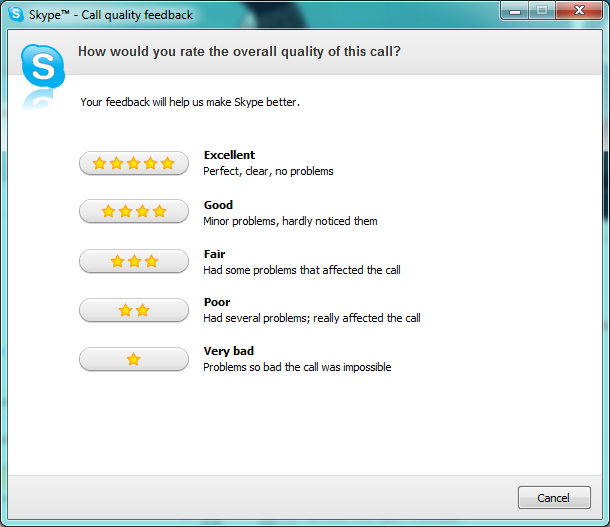
\includegraphics[trim=10px 100px 130px 25px, clip=true,scale=0.75]{figures/introduction/figures/skype.png}}
  \caption{Skype call quality rating (screenshot)}
  \label{fig:intro:fuzzy-skype}
\end{figure}

As a real-world example of fuzzy errors, consider the case of a voice
over IP service such as Skype\footnote{\url{https://www.skype.com}}.
%
After the call is made, the user can be asked to rate the quality of
the call in terms of stars: $1$ star $\rightarrow$ very bad, $5$ stars
$\rightarrow$ excellent (\Cref{fig:intro:fuzzy-skype}).
%
Intuitively, we can see that a binary error logic abstracts available
information from the diagnostic engine as a two-valued logic cannot
encode the same information as five-valued logic.

The challenge of solving this limitation is thereby twofold.
%
First, it is necessary to define an appropriate method for both
detecting and abstracting non-functional errors and the associated
error symptoms.
%
Second, it is necessary to integrate the additional knowledge in the
diagnostic process.

\researchquestion{How to encode fuzzy error
  symptoms?\label{rq:fuzzy-error-encoding}}
%
\researchquestion{How to improve \ac{SFL} to make use of the fuzzy
  error information?\label{rq:SFL-fuzzy-error-generalization}}
\subsubsection{System State}
\label{sec:intro:research-goals:system-state}

%% Problem 1: limited abstraction
A limitation of the \ac{SFL} approach presented in
\Cref{sec:intro:candidate-ranking} is related to the high level of
abstraction enforced by the usage of hit spectra as it does not
provide any information about the state of the system during each
component's execution.
%
Additionally, it abstracts the number of times each component was used
and, consequently, the sequence in which they were used in each
transaction.
%
As a consequence, hit spectrum approaches are unable to distinguishing
pairs of components for which the activity is equal.

%% Problem 2: constant gj
Furthermore, the discussed \ac{SFL} approach estimates $g_j$ as being
constant with respect to a set of observations.
%
Consider that the effective (normally unknown) goodness for component
(\eg, a hard drive) was directly related to its lifetime and took
the shape of a sigmoid, gradually decreasing over time.
%
Due to the fact that, for a hard drive, the slope of the goodness
curve is small and the time is monotonic, $g_j$ can, most of the
times, be successfully approximated by a constant with small errors.
%
However, if the observations spanned over a long period or the slope
of the goodness curve was larger (\eg, for a floppy disk), a constant
goodness function would fail to accurately model the actual goodness,
entailing large average errors.
%
Given the multiplicative nature of the goodness value usage, even
small errors can have a serious impact in the diagnosis report
ranking.

%% Problem 3: incapacity to specialize
Finally, hit spectrum approaches are not able to incorporate existent
knowledge about the system in the diagnostic process.
%
As the state of the system is completely abstracted in the hit
spectrum, it would be impossible to distinguish, for instance, a new
hard drive from an old hard drive.
%
As a consequence, even if the actual goodness curve was available for
all components in the system, the algorithm would not be able to use
it.

\researchquestion{How to enable \ac{SFL} to adapt to different systems
  based on previous diagnostic experience?\label{rq:feedback}}
%
\researchquestion{How to incorporate information about the system's
  state in \ac{SFL}?\label{rq:system-state}}


\section{Origin of Chapters}
\label{sec:intro:origin-of-chapters}
\begin{description}
\item [\Cref{sec:mhs2o,sec:mhs2p}] are
  based on the work from \citep{Cardoso14a}, which was published in
  the proceedings of \textit{the 25th International Workshop on
    Principles of
    Diagnosis}\footnote{\url{http://dx-2014.ist.tugraz.at/}} (best
  paper award). An early version of the paper was also published in
  the proceedings of both the \textit{16th Portuguese Conference on
    Artificial Intelligence
    (EPIA)}\footnote{\url{http://www.epia2013.uac.pt/}}
  \citep{Cardoso13b} and the \textit{International Conference on
    Multi-core Software Engineering, Performance, and Tools
    (MUSEPAT)}\footnote{\url{http://eventos.fct.unl.pt/musepat2013/}}
  \citep{Cardoso13c}.

\item [\Cref{sec:fuzzinel}] is based on the work from
  \citep{Cardoso14b}, which was published in the proceedings of
  \textit{the 25th International Workshop on Principles of Diagnosis}
  (best paper award nominee).

\item [\Cref{sec:nfge}] is based on the work from \citep{Cardoso13a},
  which was published in the proceedings of the \textit{27th AAAI
    Conference on Artificial Intelligence
    (AAAI)}\footnote{\url{http://www.aaai.org/Conferences/AAAI/aaai13.php}}.
\end{description}

\section{Thesis Outline}
\label{sec:intro:outline}
In \Cref{fig:intro:outline} we present the thesis outline.
%
We suggest a pre-order traversal of the tree, from top to bottom.
%




\begin{figure}[!ht]
  \begin{tikzpicture}
    [scale=1.9,
    mindmap,
    every node/.style={align=center,
      concept,
      execute at begin node=\hskip0pt,
      text=black,
      fill=white,
      line width=0.5em},
    grow cyclic,
    level 1/.append style={clockwise from=67.5,level distance=3cm,text width=3.25cm,sibling angle=135},
    level 2/.append style={clockwise from=40,level distance=2.5cm,sibling angle=80,text width=3cm,font=\small},
    level 3/.append style={clockwise from=0,level distance=2.25cm,sibling angle=45,text width=2.5cm,font=\small},]
    % \hyphenpenalty10000

    \node [text width=4cm,concept color=green!20!red] {SFL \\[0.5em] Section \ref{sec:intro:SFL}} % root
    [ concept color=green!20!red]
    child [concept color=red!90!yellow] { node {Candidate\\Generation \\[0.5em] Section \ref{sec:intro:candidate-generation}}
      child [concept color=red!80!yellow] { node  { Research\\Goals \\[0.5em] Section \ref{sec:intro:research-goals:algorithmic-efficiency}}
        child { node {\mhsII{} \\[0.5em] Chapter \ref{sec:mhs2o}} }
      }
      child [concept color=red!70!yellow] { node {Research\\Goals \\[0.5em] Section \ref{sec:intro:research-goals:horizontal-scalability}}
        child { node  {\mhsII{} \\[0.5em] Chapter \ref{sec:mhs2p}} }
      }
    }
    child [concept color=red!60!yellow] { node {Candidate\\Ranking \\[0.5em] Section \ref{sec:intro:candidate-ranking}}
      child [concept color=red!50!yellow] { node {Research\\Goals \\[0.5em] Section \ref{sec:intro:research-goals:fuzzy-errors}}
        child { node {\fuzzinel{} \\[0.5em] Chapter \ref{sec:fuzzinel}} }
      }
      child [concept color=red!40!yellow] { node {Research\\Goals \\[0.5em] Section \ref{sec:intro:research-goals:system-state}}
        child { node {\NFGE{} \\[0.5em] Chapter \ref{sec:nfge}} }
      }
    };
  \end{tikzpicture}
  \caption{Thesis outline\label{fig:intro:outline}}
\end{figure}
